\chapterimage{chapter_head_2.pdf} % Chapter heading image

\chapter{Física - Termologia}

\section{Escalas temométricas}\index{Escalas termométricas}
As escalas mais conhecidas (Celsius e Fahrenheit) foram construídas usando, basicamente, a transição de estados da água: fusão e ebulição. A escala Kelvin (escala absoluta) também pode ser definida como segue:

\begin{table}[!h]
    \centering
    \caption{Escalas mais conhecidas e seus valores para os pontos de fusão e ebulição da água}
    \vspace{.5cm}
    \label{tab:my-table}
    \begin{tabular}{cccc}
    \textbf{Escala}                    & \textbf{Celsius {[}°C{]}} & \textbf{Fahrenheit {[}°F{]}} & \textbf{Kelvin {[}K{]}} \\
    \textbf{Ponto de ebulição da água} & 100                       & 212                          & 373,15                  \\
    \textbf{Ponto de fusão da água}    & 0                         & 32                           & 273,15                 
    \end{tabular}
\end{table}


\begin{figure}[!h]
    \caption{Representação das escalas termométricas}
    
    \centering % para centralizarmos a figura
    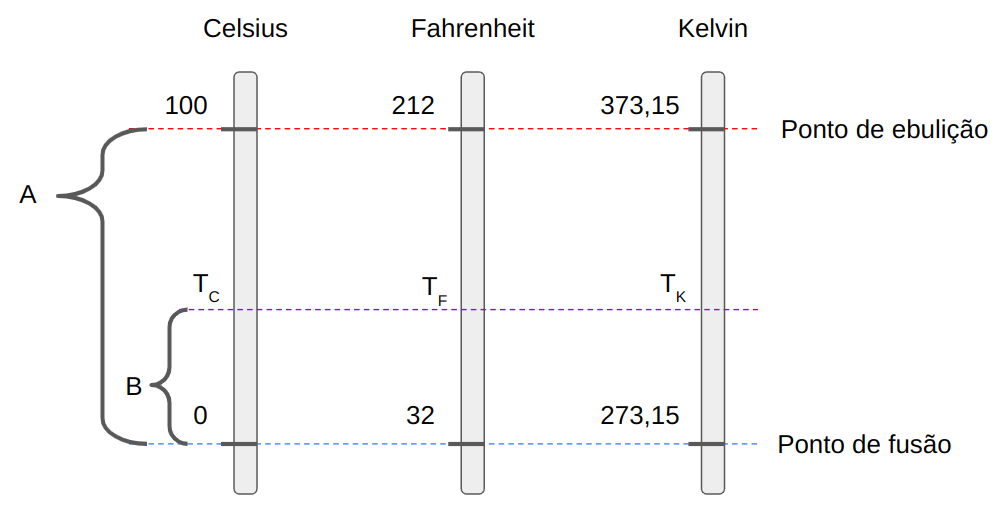
\includegraphics[width=12cm]{Pictures/FISICA_EM/TERMOLOGIA/escalas_termometros.png} % leia abaixo
    \label{figura:qualquernome}
\end{figure}

Como pode ser visto na figura acima, é possível estabelecer relações entre as escalas de modo a converter as temperaturas. Uma forma de estabelecer as conversões entre as escalas é fazer a proporção entre as razões $A/B$ de cada escala, assim:

\begin{ceqn}
\begin{align*}
    \frac{T_C - 0}{100 - 0} = \frac{T_F - 32}{212 - 32} = \frac{T_K-273,15}{373,15 - 273,15}
\end{align*}
\begin{align*}
    \frac{T_C}{100} = \frac{T_F - 32}{180} = \frac{T_K-273,15}{100}
\end{align*}
\end{ceqn}

Através da relação acima, é possível relacionar as escalas e fazer a conversão entre elas, como segue:

\subsection{Relação entre Celsius e Fahrenheit}\index{Relação entre Celsius e Fahrenheit}
\begin{ceqn}
    \begin{align*}
        \frac{T_C}{100} &= \frac{T_F - 32}{180} \\
        \frac{180 \cdot T_C}{100} &= T_F -32 \\
        \frac{9}{5} \cdot T_C &= T_F-32 \\
    \end{align*}
\end{ceqn}

\subsection{Relação entre Celsius e Kelvin}\index{Relação entre Celsius e Kelvin}
\begin{ceqn}
    \begin{align*}
        \frac{T_C}{100} &= \frac{T_K-273,15}{100} \\
        T_C&=T_K-273,15 \\
    \end{align*}
\end{ceqn}

\subsection{Relação entre Fahrenheit e Kelvin}\index{Relação entre Fahrenheit e Kelvin}
\begin{ceqn}
    \begin{align*}
        \frac{T_F - 32}{180} &= \frac{T_K-273,15}{100} \\
        \frac{100}{180}\cdot (T_F-32) &= T_K-273,15 \\
        \frac{5}{9} \cdot (T_F-32) &= T_K-273,15 \\
    \end{align*}
\end{ceqn}

\begin{example}
Calcule a temperatura em graus Fahrenheit sabendo que a temperatura em ${}^\text{o}$C é de 32.

\begin{ceqn}
\begin{align*}
\frac{9}{5} \cdot T_C =& T_F - 32 \\
\frac{9}{5} \cdot 32 =& T_F - 32 \\
1,8 \cdot 32 =& T_F - 32 \\
57,6 =& T_F -32 \\
T_F =& 57,6 + 32 \\
T_F =& 89,6 {}^oF \\
\end{align*}
\end{ceqn}
\end{example}
